
\documentclass[conference]{IEEEtran}
\usepackage{blindtext, graphicx}
\usepackage[T1]{fontenc}
\usepackage[utf8x]{inputenc}
\usepackage{spverbatim}
\newcommand{\shellcmd}[1]{\\\indent\indent\texttt{\footnotesize\$ #1}\\}

% *** GRAPHICS RELATED PACKAGES ***
%
\ifCLASSINFOpdf
  % \usepackage[pdftex]{graphicx}
  % declare the path(s) where your graphic files are
  % \graphicspath{{../pdf/}{../jpeg/}}
  % and their extensions so you won't have to specify these with
  % every instance of \includegraphics
  % \DeclareGraphicsExtensions{.pdf,.jpeg,.png}
\else
  % or other class option (dvipsone, dvipdf, if not using dvips). graphicx
  % will default to the driver specified in the system graphics.cfg if no
  % driver is specified.
  % \usepackage[dvips]{graphicx}
  % declare the path(s) where your graphic files are
  % \graphicspath{{../eps/}}
  % and their extensions so you won't have to specify these with
  % every instance of \includegraphics
  % \DeclareGraphicsExtensions{.eps}
\fi
% graphicx was written by David Carlisle and Sebastian Rahtz. It is
% required if you want graphics, photos, etc. graphicx.sty is already
% installed on most LaTeX systems. The latest version and documentation can
% be obtained at: 
% http://www.ctan.org/tex-archive/macros/latex/required/graphics/
% Another good source of documentation is "Using Imported Graphics in
% LaTeX2e" by Keith Reckdahl which can be found as epslatex.ps or
% epslatex.pdf at: http://www.ctan.org/tex-archive/info/
%
% latex, and pdflatex in dvi mode, support graphics in encapsulated
% postscript (.eps) format. pdflatex in pdf mode supports graphics
% in .pdf, .jpeg, .png and .mps (metapost) formats. Users should ensure
% that all non-photo figures use a vector format (.eps, .pdf, .mps) and
% not a bitmapped formats (.jpeg, .png). IEEE frowns on bitmapped formats
% which can result in "jaggedy"/blurry rendering of lines and letters as
% well as large increases in file sizes.
%
% You can find documentation about the pdfTeX application at:
% http://www.tug.org/applications/pdftex


% correct bad hyphenation here
\hyphenation{op-tical net-works semi-conduc-tor}


\begin{document}
%
% paper title
% can use linebreaks \\ within to get better formatting as desired
\title{LINGI1341 - Analyse de site web\\Projet 2 - www.bbc.com}


% author names and affiliations
% use a multiple column layout for up to three different
% affiliations
\author{\IEEEauthorblockN{Guillaume Calmant}
\IEEEauthorblockA{Université Catholique de Louvain\\ Sciences informatiques\\
NOMA : 62991200\\
Email: guillaume.calmant@student.uclouvain.be}
}

%%%%%%%%%%%%%%%%%%%%%%%%%%%%%%%%%%%%
%TODO : 
% - HTTP version (http)
% - public resolver (dns)
% - revoir footnotes
% - cmp header fields (http)
% - uncommon records (dns)
% - tls and dnssec

% make the title area
\maketitle


\begin{abstract}
This paper has been written for the course of \textit{Computer networks : information transfer
} teached by Pr. \textit{Olivier Bonaventure} at \textit{EPL}, the polytechnics school of \textit{UCL}. We were asked to analyze a website chose among others, with some criteria.  
%\boldmath
\end{abstract}
% IEEEtran.cls defaults to using nonbold math in the Abstract.
% This preserves the distinction between vectors and scalars. However,
% if the journal you are submitting to favors bold math in the abstract,
% then you can use LaTeX's standard command \boldmath at the very start
% of the abstract to achieve this. Many IEEE journals frown on math
% in the abstract anyway.

% Note that keywords are not normally used for peerreview papers.
%\begin{IEEEkeywords}
%IEEEtran, journal, \LaTeX, paper, template.
%\end{IEEEkeywords}






% For peer review papers, you can put extra information on the cover
% page as needed:
% \ifCLASSOPTIONpeerreview
% \begin{center} \bfseries EDICS Category: 3-BBND \end{center}
% \fi
%
% For peerreview papers, this IEEEtran command inserts a page break and
% creates the second title. It will be ignored for other modes.
\IEEEpeerreviewmaketitle



\section{Introduction}
%%%%%%%%%%%%%%%%%%%%%%%%%%%%%%%%%%%%%%
    The British Broadcasting Corporation \footnote{\textit{B.B.C.}} is a public service broadcaster located in London. Founded in 1922, the domain of the service was registered in 1994 and the website launched in 1997. To inspect this website, we are going to, firstly, to analyze the \textit{HTTP} traffic. Furthermore, we will perform a \textit{DNS} analysis, followed by an examination of the \textit{TCP} use on the website to conclude with the \textit{DNSSEC} and the \textit{TLS} protocols. 
    
    %                T O                                                                        D O                         % 
    %%%%%%%%%%%%%%%%%%%%%%%%%%%%%%%%%%%%%%%%%%%%%%%%%%%%%%%%%%%%%%%%%%%%%%%%%%%%%%%%%%%%%%%%%%%%%%%%%%%%%%%%%%%%%%%%%%%%%%%%
    %TODO :CDN is a special network designed to cache content, so that usr request served faster + to unload origin servers.%
    %%%%%%%%%%%%%%%%%%%%%%%%%%%%%%%%%%%%%%%%%%%%%%%%%%%%%%%%%%%%%%%%%%%%%%%%%%%%%%%%%%%%%%%%%%%%%%%%%%%%%%%%%%%%%%%%%%%%%%%%
    
%public brodcaster fondé en situé à, sur internet depuis. Les analyse qu'on va faire.

%% Domaines


\section{HTTP}


\subsection{Domains}
With an empty cash, using \textit{Chrome} 62.0.3202.89 for \textit{Linux}, we can notice the fast display of the content, inducing certainly a use of \textit{CDNs}\footnote{\textit{Content Delivery Network, per example \textit{fastly} & \textit{akamai}, used by the website}, uses to enhance the performances delivering data geographically}, because of the amount of medias presents on the homepage. Thanks to the network inspector we can go deeply, even produce a \textit{HAR}\footnote{http://www.softwareishard.com/blog/har-12-spec/} file and reveal more than seventy-five different domains contacted in order to display the index. These domains are mainly reached to call scripts, load some medias (images, videos, graphics,...) and harvest analytic data. We will provide the listed domains contacted. 

As you can see in annexes, \textit{fig 1}, many of the domains are contacted to harvest analytic data or broadcast images. The analytic part is done by different ways, in example the scripts collect data trough adds \footnote{per example with \textit{adexchange}}, videos, images and sometimes games. The data is useful for the broadcaster to enhance the performance of the website, deliver more pertinent and cheaper advertisements\footnote{Many services proposed to the website managers work on an auction system for using adds}, have a better knowledge of their users  and how their data is distributed in the world. In example, one of the technologies used by \textit{bbc}, developed by \textit{Drawbridge}, can guess if different users consult the website on the same device\footnote{adsymptotic.com}. Other enhancements are performed, two connections can be opened when the broadcaster call a domain; some service propose cookies to \textit{sniff} the client's connection\footnote{effecctivemeasure.net}, collecting per example data on what website he visited, which was its title, IP address, ... \footnote{seb.scorecardresearch.com}; etc. All the data is kept\footnote{\textit{"up to 90 days. When it is aggregated to observe trends, it may be used for analytic purposes indefinitely."} (http://www.effectivemeasure.com/privacy-policy/)}, compute and used thanks to diverse techniques of data mining \footnote{\textit{static.adsafeprotected.com}} \footnote{https://www.headerdirect.com} \footnote{https://www.stackadapt.com/privacy}. All the cookies used by \textit{bbc} is listed and detailed at this link: \textit{http://www.bbc.com/usingthebbc/cookies/how-does-the-bbc-use-cookies/}. 
 
 
 %Sometimes aim on tablet or phone 



%%%%%%%%%%%%%%%%%%%%%%%%%%%%%%%%%%%%%%%% Ressources
\subsection{Resources}
For example,we analyze the homepage, 
%liste de tous les types de ressources (html, cc, javascript, flash, …) qui sont utilisées sur votre site web. Certains navigateurs peuvent exporter dans le format HAR une page web visualisée et il existe des outils pour analyser ce format HAR
Between 130 and 500 (1.2 MB up to 3.6 MB) requests performed depending of the cache, the path,re-transmissions,scroll ,... 
For a time varying from approximately 2sec (from London, UK with cached data) up to 21sec (Vancouver, Canada with an empty cache). 
Behind this analysis we can highlight the fact that there is a bad optimization of the resources distributed on this page. It may come from cached elements and render blocking elements (directly impacting on the \textit{DOM} contents loaded) because of the loading time contrast. 

From our \textit{HAR} file with no cached elements we can list the resources : 

\begin{table}[h!]
     \centering
     \begin{tabular}{|c|c|c|}
        \hline
        
        Object & size (in KB) & Requests 
    \\
        \hline
        Image & 1200 & 81 \\
        HTML & 871.9 & 18 \\
        Script & 647.1 & 58 \\
        CSS & 75.3 & 10 \\
        Other & 6.7 & 6 \\
        TOTAL & 3600 &  173 \\
        \hline
    \end{tabular}
     %\caption{}
     \label{tab:my_label}
 \end{table}
 
 Clearly, the important number of images and elements are slowing down the display of the page\footnote{fig 8}. We can improve this by more compressing images, combining and minifying scripts and enhancing how the data is cached (in the browser). Some of the static have no, or small, \textit{max-age} or \textit{expires} flags value set. It's sometimes due to the analytic and the need of fresh data, however there's no reason for the \textit{favicon}, for example, to expires in \textit{11.1} hours. 
 
 Furthermore, render blocking scripts slow down the \textit{DOM} construction\footnote{fig 9}. Many third-party, and internal\footnote{\textit{bbccookies}}, script call \textit{Document.write} and this should be avoid using asynchronously \textit{javascript}\footnote{\textit{https://github.com/krux/postscribe}}. 
 

 %https://developer.mozilla.org/en-US/docs/Web/Events/DOMContentLoaded
 
%already highlighted : use of non standard http fields, (no-cache) X-cache:HIT means that your request was served by CDN, not origin servers.
%\footnote{https://cdn.uclouvain.be/groups/cms-editors-ingi/lingi1341-rapports/bbc.pdf} 

%https://modernizr.com/ compatibility browsers (old ...) 

%style orb for customizable pivot table control http://orbjs.net/, cta to "animate your "action-to-effect" paths." (Navigation in tile based apps, buttons, sidebars, ...) https://kushagragour.in/lab/ctajs/  
% Policy show prompt https://github.com/macmladen/lucar/blob/master/assets/sample_html5/bbc.html window.orb
%cookies are sent when policy accepted (even if not ?)

\subsection{TCP ports}
With the use of \textit{tcpsnitch}\footnote{https://github.com/GregoryVds/tcpsnitch} we can retrieve a \textit{.pcap} file from a \textit{firefox}\footnote{Version 57.0.1 (64 bits) for Ubuntu} session and perform analyses about the \textit{tcp} ports used thanks to \textit{Wireshark}\footnote{Version 2.2.6}. On this website the only used ports are \textit{80} and \textit{443}. 

\subsection{HTTP requests and responses}

\textit{HTTP} uses \textit{TCP} to transfer data, accessing servers thanks to an address trough a port. Some ports are reserved for a range of applications, including \textit{HTTP}. The most used ports for \textit{http} are, 80, 443 (https) and 8080 (webcache).\footnote{Other reserved ports : 9443, 10011 and 11371} BBC's webserver uses \textit{HTTP/1.1}\footnote{https://tools.ietf.org/html/rfc2616}, by default using a \textit{keep-alive} connection. Thanks to the previous retrieved \textit{.pcap} files we can observe the \textit{tcp} traffic and so the \textit{http} requests and responses. 

\subsection{Non-standard and special use of headers}
\begin{itemize} %vary ? & Content type ? 

    \item \textbf{X-Cache}: this header is used to inform if a requested file is found or not, cached, in a \textit{CDN} per example. \textit{X-Cache}: HIT means that the requested file was served from cache and MISS a not served file. Other \textit{Varnish}\footnote{https://varnish-cache.org/} headers are used to deal with the cached data, as \textit{X-Cache-Hits}, \textit{X-Cache-Age}, \textit{X-Cache-Action},... . 
    
    \item \textbf{Access-Control-Allow-Origin}: 
    Header from CORS\footnote{https://developer.mozilla.org/en-US/docs/HTTP/Access\_control\_CORS}, standing for \textit{cross-origin resource sharing}, permit to build a web-page while performing \textit{cross-site} \textit{HTTP} requests. That means we can retrieve, per example, an image from a \textit{CDN}, text from our personal server and other resources from different domains. This header in particular \textit{"indicates whether the response can be shared with resources with the given origin."}\footnote{https://developer.mozilla.org/en-US/docs/Web/HTTP/Headers/Access-Control-Allow-Origin} \footnote{https://www.w3.org/TR/cors/\#resource-implementation} The wildcard value is not a problem if the cross domain policy is well configured.\footnote{http://www.bbc.com/crossdomain.xml} The real question is can I trust these domains and are they secured.\footnote{http://blog.h3xstream.com/2015/04/crossdomainxml-beware-of-wildcards.html} 
    
    \item \textbf{X-PAL-Host}: indicating an address, pal138.back.live.telhc.local:80. After some researches, we find a post\footnote{http://narkive.com/sn0WOxkE} written by \textit{Tom Pride}\footnote{https://www.linkedin.com/in/tompride1}, who perform multiple works for the \textit{bbc}. In this post, Tom asks for help while configuring \textit{DRDB}\footnote{https://docs.linbit.com/} nodes for the \textit{bbc} and paste his configuration file. Thanks to this we can collect more information on the \textit{bbc}'s servers. We can firstly observe some addresses assigned to nodes: \textit{172.23.8.69} and \textit{172.23.8.70}. According to \textit{rfc1918}\footnote{https://tools.ietf.org/html/rfc1918} these are addresses for private internets.
    
    \textit{DRDB} stands for \textit{Distributed Replicated Block Device} and is used to link and synchronize by replication some devices as nodes of the network. \footnote{see fig 10} Furthermore, thanks to \textit{heartbeat}\footnote{http://linux-ha.org/wiki/Heartbeat}, when a server experience errors the second server take automatically its role.
    
    "Tom, ... Please don't paste inline this time, ..."\footnote{https://lists.gt.net/linuxha/pacemaker/75542} \footnote{https://cwe.mitre.org/data/definitions/200.html}
    
    \item \textbf{x-amz-...}: headers use by Amazon Simple Storage Service thanks to deliver files.\footnote{http://docs.aws.amazon.com/AmazonS3/latest/API/Welcome.html}. 

    \item \textbf{Vary} : indicates that a server response is based on the \textit{Origin} header. (Origin, X-CDN, ...) 
    
    \item \textbf{X-Fastly-...}: headers from \textit{Fastly} \textit{CDN}.\footnote{https://docs.fastly.com/guides/api-caching/implementing-api-cache-control}  

\end{itemize}
%les informations non-standard qui pourraient se trouver dans la requête (essayez d’expliquer leur rôle)

We may see here some problems concerning the security and the lack of certain headers, but we can see the missing headers on credentials data:\footnote{after logged in even more headers are used} 

    \begin{itemize}
        \item \textit{X-Frame-Options: DENY}: "indicates a policy that specifies whether the browser should render the transmitted resource within a <frame> or an <iframe>."\footnote{https://tools.ietf.org/html/rfc7034#page-4}
        \item \textit{X-Content-Type-Options: nosniff}: "indicate that the MIME types advertised in the Content-Type headers should not be changed and be followed."\footnote{https://developer.mozilla.org/fr/docs/Web/HTTP/Headers/X-Content-Type-Options}
        \item \textit{x-permitted-cross-domain-policies:none} "instructs Flash and PDF files that they should read"\footnote{https://danielnixon.org/http-security-headers/}, here, none cross domain policies. 
        \item \textit{x-xss-protection:1; mode=block}: "stops pages from loading when they detect reflected cross-site scripting (XSS) attacks."\footnote{https://developer.mozilla.org/en-US/docs/Web/HTTP/Headers/X-XSS-Protection} 
        \item \textit{cache-control:no-cache,private,no-store}: used to define the cache policies. 
        \item \textit{strict-transport-security:max-age=31536000}: to force the use of \textit{https} during the \textit{max-age} time.
        \item \textit{P3P:policyref= }: to define the \textit{P3P} policies.\footnote{https://www.w3.org/2002/04/P3Pv1-header.html}
        ...
    \end{itemize}

%Ne limitez pas votre analyse à la première page du site web. Essayez de faire un petit scenario d’utilisation qui permet au site d’apprendre quelque chose sur vous (langue préférée, vote en ligne, login avec username/password). Si le site contient une partie “e-commerce”, essayez de remplir votre caddie virtuel et allez jusqu’à l’étape du paiement, ce sera intéressant pour l’analyse de la partie consacrée à la sécurité.

%Durant votre analyse, essayez de vous concentrer sur les choses qui sont inattendues et essayez de les comprendre. Cela nécessitera probablement quelques recherches, mais vous permettra de renforcer votre connaissance des réseaux.

\section{DNS}
Thanks to \textit{dig} and \textit{nslookup} commands, \textit{dnsmap}\footnote{https://github.com/makefu/dnsmap} tool and \textit{.pcap} files we can perform analysis on the \textit{DNS} records and traffic.
%28.pcap 31 32 33 37 42 48 53 54 55 58 59 62 64 66 68 70 71 76 79 80 82 85 86 87 88 95 96 98 99 100 102 106 109 112 116 124 126 127 130 131 132 135 138 141 142 148 150 152 154 156 


%Vous pouvez utiliser dig ou nslookup en ligne de commande pour interroger le DNS. Il existe aussi de nombreuses librairies que vous pouvez exploiter à cette fin. Pour faire des requêtes DNS, vous pouvez utiliser des resolvers DNS publics, en voici quelques uns : https://moodleucl.uclouvain.be/mod/page/view.php?id=532433

\subsection{Domains} 
%- Quels sont les serveurs DNS (records NS) qui supportent ce domaine. Sont-ils accessibles en IPv4 et IPv6 ou seulement via un des deux protocoles ?
\begin{table}[h!]
     \centering
     \begin{tabular}{|c|c|c|}
        \hline
        
         Name servers & IPv4 & IPv6 
    \\
        \hline
        ns4.bbc.net.uk & 156.154.65.17 & 2610:a1:1014::17 \\
        ns3.bbc.co.uk & 156.154.66.17 & 2610:a1:1015::17 \\
        ns4.bbc.co.uk & 156.154.67.17 & 2001:502:4612::17 \\
        ns3.bbc.net.uk & 156.154.64.17 & 2001:502:f3ff::17 \\
        \hline
    \end{tabular}
     %\caption{}
     \label{tab:my_label}
 \end{table}
 Listed above the severs authoritative for the zone \textit{ns.bbc.co.uk}. The start of authority reports a responsible, \textit{hostmaster.bbc.co.uk}, a serial changing when the domain is updated, \textit{2017101601}, the number of seconds before the \textit{NS} servers should update their serial numbers, \textit{1800},  the number of seconds before the \textit{NS} servers should update their serial numbers if previously failed \textit{600}, the number of seconds after which the \textit{NS} expires and the \textit{TTL} or \textit{minimum} field. According to \textit{rfc2308}\footnote{https://tools.ietf.org/html/rfc2308} this field \textit{"has been overloaded in the past to have three
   different meanings"} and is now the time to cache a negative response.


\subsection{TTL}
Each record has its own \textit{TTL}, the time in seconds, after which the record is refreshed. Thus a small \textit{TLL} ensures that if a record is invalid, it will not stay too long. We can observe that \textit{BBC}'s records have really short \textit{TTL}, 5 (for A and MX records) or 15 minutes (for any else record). It can be short for multiple reasons, avoiding cache poisoning is a good one since the broadcaster has been targeted by \textit{DDoS} attacks he's surely concerned by \textit{DNS} attacks. However, \textit{DNSSEC} is not set and thus these \textit{TTL}s are maybe not set for a security purpose. Nevertheless a short \textit{TTL} is recommended for a \textit{DNS} fail-over\footnote{https://www.dynu.com/DNS-Failover} mechanism, which is clearly in the spirit of \textit{Linux-HA} and \textit{DRBD}. Shorter \textit{TTL} for \textit{A} and \textit{MX} records are set certainly because, on one hand \textit{IPv4} is still more used than \textit{IPv6} and on the other hand \textit{BBC} surely wants to be easily reached by mails. We can remark the \textit{Pride} has also implemented the \textit{squid-cache} proxy technology reducing bandwidth and response time. 


%In the 
%AKAMAI
%AMAZONE
%VERIZON (edgecast)
%RUBICONPROJECT 
%COMODOCDN
%2MDN.net 


%ocsp.pki.goog: type A, class IN   : OCSP proto to validate a key 
%& comodo 


\subsection{Records}

\begin{table}[h!]
     \centering
     \begin{tabular}{|c|c|c|}
        \hline
        
        Record type & name & value
    \\
        \hline
        MX & cluster8.eu.messagelabs.com & 85.158.137.99\\
        MX & cluster8.eu.messagelabs.com & 85.158.137.19\\
        MX & cluster8.eu.messagelabs.com & 85.158.140.211\\
        MX & cluster8.eu.messagelabs.com & 85.158.140.195\\
        MX & cluster8.eu.messagelabs.com & 85.158.139.51\\
        MX & cluster8.eu.messagelabs.com & 85.158.139.35\\
        MX & cluster8.eu.messagelabs.com & 85.158.139.19\\
        MX & cluster8a.eu.messagelabs.com & 85.158.139.103\\
        A & bbc.com & 212.58.246.78\\
        A & bbc.com & 212.58.246.79\\
        A & bbc.com & 212.58.244.22\\
        A & bbc.com & 212.58.244.23\\
        AAAA & bbc.com & 2001:41c1:4008::bbc:2\\
        AAAA & bbc.com & 2001:41c1:400c::bbc:1\\
        AAAA & bbc.com & 2001:41c1:400c::bbc:4\\
        AAAA & bbc.com & 2001:41c1:4008::bbc:3\\
        AAAA & bbc.com & 2001:41c1:4008::bbc:4\\
        AAAA & bbc.com & 2001:41c1:400c::bbc:3\\
        AAAA & bbc.com & 2001:41c1:4008::bbc:1\\
        AAAA & bbc.com & 2001:41c1:400c::bbc:2\\
        SOA & ns.bbc.co.uk & 132.185.161.100\\
        NS & ns4.bbc.net.uk & 156.154.65.17\\
        NS & ns4.bbc.net.uk & 2610:a1:1014::17\\
        NS & ns3.bbc.co.uk & 156.154.66.17\\
        NS & ns3.bbc.co.uk & 2610:a1:1015::17\\
        NS & ns4.bbc.co.uk & 156.154.67.17\\
        NS & ns4.bbc.co.uk & 2001:502:4612::17\\
        NS & ns3.bbc.net.uk & 156.154.64.17\\
        NS & ns3.bbc.net.uk & 2001:502:f3ff::17\\
        TXT & bbc.com & MS=ms25863558\\
        TXT & bbc.com & Fzj91DPhHcxL3FxKMiBraJ9CajRin4nqr8...\\
        TXT & bbc.com & dropbox-domain-verification=mtgv0f2pudoz\\
        \hline
    \end{tabular}
     %\caption{}
     \label{tab:my_label}
 \end{table}
 
 The \textit{TXT} records are here used to perform domain validations on keys given for three different services \textit{Microsoft Office 365}, \textit{Amazon SES} and \textit{Dropbox Business}. 
 
 \subsection{Other records}
 Other records can be retrieve in the \textit{DNS} analysis, such as the \textit{SPF} record which stand for sender policy framework. It's an email-validation system ton avoid spamming, spoofing, injecting, etc.\footnote{https://tools.ietf.org/html/rfc7208}
\textit{SPF v=spf1 ip4:212.58.224.0/19 ip4:132.185.0.0/16 ip4:78.136.53.80/28 ip4:78.136.14.192/27 ip4:78.136.19.8/29 ip4:89.234.10.72/29 ip4:74.112.66.33 ip4:208.251.80.51 ip4:89.202.185.0/24 ip4:207.159.133.98 ip4:207.159.133.99 include:msgfocus.com include:cmail1.com include:mktomail.com include:servers.mcsv.net include:redsnapper.net ?all}

Contained in another \textit{TXT} record, we can find the \textit{SPF} record. \begin{itemize}
\item\textit{TXT bbc.com v=spf1 ip4:212.58.224.0/19 ip4:132.185.0.0/16 ip4:78.136.53.80/28 ip4:78.136.14.192/27 ip4:78.136.19.8/29 ip4:89.234.10.72/29 ip4:74.112.66.33 ip4:208.251.80.51 ip4:89.202.185.0/24 ip4:207.159.133.98 ip4:207.159.133.99 include:msgfocus.com include:cmail1.com include:mktomail.com include:servers.mcsv.net include:redsnapper.net ?all}.
\end{itemize}

The last record found is the \textit{SRV} informing on the servers services.\footnote{https://tools.ietf.org/html/rfc2782}

 \begin{itemize}
\item\textit{SRV \_sip.\_tls.bbc.com sip.bbc.com 207.82.79.70 443 0
SRV \_sip.\_tls.bbc.com sip.bbc.com 207.82.79.73 443 0
SRV \_xmpp-server.\_tcp.bbc.com sip.bbc.com 207.82.79.70 5269 0
SRV \_xmpp-server.\_tcp.bbc.com sip.bbc.com 207.82.79.73 5269 0
SRV \_sipfederationtls.\_tcp.bbc.com sip.bbc.com 207.82.79.70 5061 0
SRV \_sipfederationtls.\_tcp.bbc.com sip.bbc.com 207.82.79.73 5061 0}
 \end{itemize}
 
 \subsection{Sub-domains}
 With the use of the brute-force tool \textit{dnsmap} we can identify more sub-domains than already known from \textit{bbc.com}, listed below. Two of these revealed us an internal \textit{ip} which can be seen as an information exposure.\footnote{https://cwe.mitre.org/data/definitions/200.html}
 \begin{itemize}
     \item as.bbc.com : IPv4 address \#1: 132.185.162.193.
     \item av.bbc.com : IPv4 address \#1: 207.82.79.75, IPv4 address \#2: 207.82.79.72.
     \item beta.bbc.com : IPv4 address \#1: 212.58.244.82, IPv4 address \#2: 212.58.246.113.
     \item li.bbc.com : IPv4 address \#1: 95.182.253.49, IPv4 address \#2: 95.182.253.48.
     \item m.bbc.com : IPv4 address \#1: 212.58.246.173, IPv4 address \#2: 212.58.244.162.
     \item mobile.bbc.com : IPv4 address \#1: 212.58.246.186, IPv4 address \#2: 212.58.244.29.
     \item sandbox.bbc.com : IPv4 address \#1: 192.168.193.10. 
     \item search.bbc.com : IPv4 address \#1: 212.58.246.160, IPv4 address \#2: 212.58.244.157.
     \item shop.bbc.com : IPv4 address \#1: 207.159.133.98.
     \item test.bbc.com : IPv4 address \#1: 212.58.228.13, IPv6 address \#1: 2001:41c1:4008:d::bbc:88, IPv6 address \#2: 2001:41c1:4008:d::bbc:89.
     \item tv.bbc.com : IPv4 address \#1: 104.120.249.95.
     \item webmail.bbc.com : IPv4 address \#1: 132.185.162.192.
     \item www.bbc.com : IPv4 address \#1: 212.58.246.95, IPv4 address \#2: 212.58.244.71.
     \item localhost.bbc.co.uk : IPv4 address \#1: 127.0.0.1.\footnote{https://www.acunetix.com/vulnerabilities/web/same-site-scripting}
     \item er.bbc.co.uk : IPv4 address \#1: 10.72.136.19.\\
     ... 
 \end{itemize}
%- Les serveurs HTTP que vous contactez sont ils accessibles en IPv4 (records A) et/ou IPv6 (records AAAA) ?

%\textbf{idem inside ucl ?}
%- Les adresses retournées par ces serveurs sont-elles les mêmes depuis votre domicile, le réseau de l’UCL ou des resolvers DNS publics (cfr information ci-dessous) ?

%\textbf{CNAME allias}
%- Observez-vous une utilisation d’alias (records CNAMEs) ?

%\textbf{other records ?}
% - Le DNS contient-ils d’autres types de records DNS que les records traditionnels ? Si oui, quels sont-ils et à quoi peuvent-ils bien servir ?




%Quel est le TTL des réponses DNS que vous recevez ? Est-il le même pour tous les types de records ? Pourquoi ?
% Les resolvers que vous contactez pour obtenir un record A/AAAA retournent-ils toujours la même adresse ou observez-vous un partage de charge entre plusieurs serveurs (cela pourrait vous amener à découvrir quel CDN est utilisé par votre site web)?
%Le DNS contient-ils d’autres types de records DNS que les records traditionnels ? Si oui, quels sont-ils et à quoi peuvent-ils bien servir ?
% other 

\section{TCP}
Again the retrieved files with the help of \textit{tcpsnitch} will help us to perform analyzes. Also we add to \textit{wireshark} the \textit{tcp.flags.reset==1 or tcp.flags.fin==1} filter to have a better sketch of the used \textit{tcp} connections. So we can observe only one connection to \textit{bbc.com} and five simultaneous \textit{tcp} connections when communicating to an \textit{akamai} server.\footnote{see fig 11} To learn more about the options used by \textit{tcp} protocol on the \textit{BBC} website, we can make further investigations using \textit{tracebox}\footnote{http://www.tracebox.org}. Performing these analysis highlights the fact that the \textit{tcp} protocol on the broadcaster side is the most basic version of \textit{tcp}. It does not implements the padding, the fast open or the explicit congestion notification option. So basically it only supports window scale, timestamps and selective acknowledgements. Also during the research we noticed that each connection terminate with the \textit{FIN} bit set and not the \textit{RST}.


\section{TLS and DNSSEC}
As previously seen the \textit{DNSSEC} is not configured for \textit{bbc.com}\footnote{see fig 12}, confirmed by \textit{Verisign labs}\footnote{http://dnssec-debugger.verisignlabs.com}.
For \textit{TLS}, \textit{SSL Labs}\footnote{https://www.ssllabs.com/ssltest} give a grade of \textit{A} for every tested addresses. The broadcaster uses \textit{TLS v1.2}\footnote{not vulnerable to CVE-2014-3566} and thanks to \textit{OpenSSL} we can ask the certificate.  Then we retrieve multiple information in the \textit{SSL} certificate, for example the \textit{British Broadcasting Corporation} has the serial \textit{18EBFFD5FE552205E9EE29DB} and the fingerprint \textit{E14E0B9F8C3F3BA7A2F0F2C6ECCE8983C38349955ED591
964275A18D61129171}. Using the protocol versions and features, we can inform us on what is supported by the server. It only supports \textit{secure renegotiation} and \textit{downgrade protection} features and has a weak \textit{triple data encryption}. To conclude this section, it does not support compression and may be vulnerable to \textit{CRIME}\footnote{https://cve.mitre.org/cgi-bin/cvename.cgi?name=cve-2012-4929}.   

\section{Conclusion}
The British broadcaster uses multiple \textit{CDN}s in order to deliver information in an efficiently manner to his public and also make a lot of analytic to enhance the visit of the users on the website. We have seen the impact of resources on a the the loading of a page and the importance of avoiding render blocking elements. We listed and detailed some non-standard headers and special use of generic headers, discovering some technologies implemented on the web-server and much more. Then we performed a \textit{DNS} detailing some records and reveal internals \textit{ip}s. \textit{TCP} section has mainly highlights the possibility of a browser and a server to communicate trough simultaneous \textit{TCP} connections. We finally noticed some potentially weaknesses trough the \textit{TLS} paragraph and remind the importance of paying attention even in a "secure" protocol. 

\section{Annexes}
\begin{figure}
\caption{Domains contacted for the index page (excluding domains belonging to \textit{bbc})}
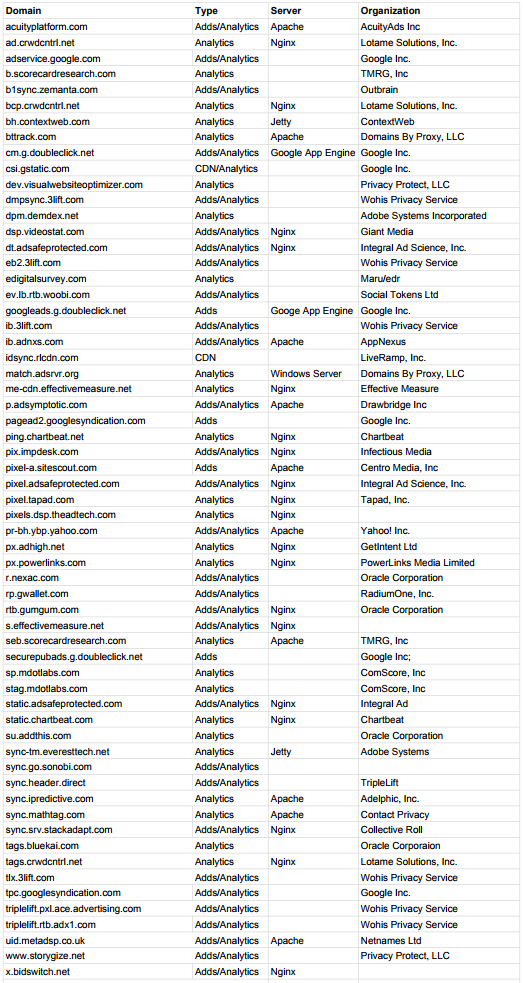
\includegraphics[width=\linewidth]{domains.png}
\end{figure}

\begin{figure}
\caption{Oracle Data Cloud services \\ (http://www.bluekai.com/consumers\_howdoesitwork.php)}
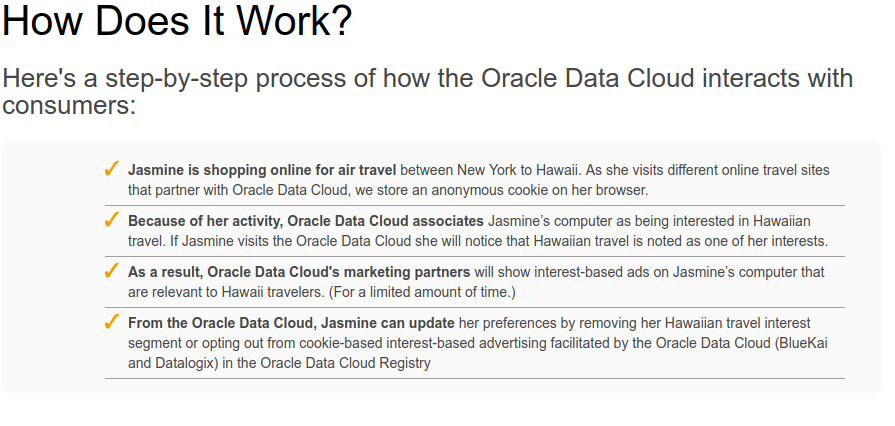
\includegraphics[width=\linewidth]{Oracle.png}
\end{figure}

%192.168.112.2O7.net

\begin{figure}
\caption{Storygize solutions \\ (http://www.storygize.com/)}
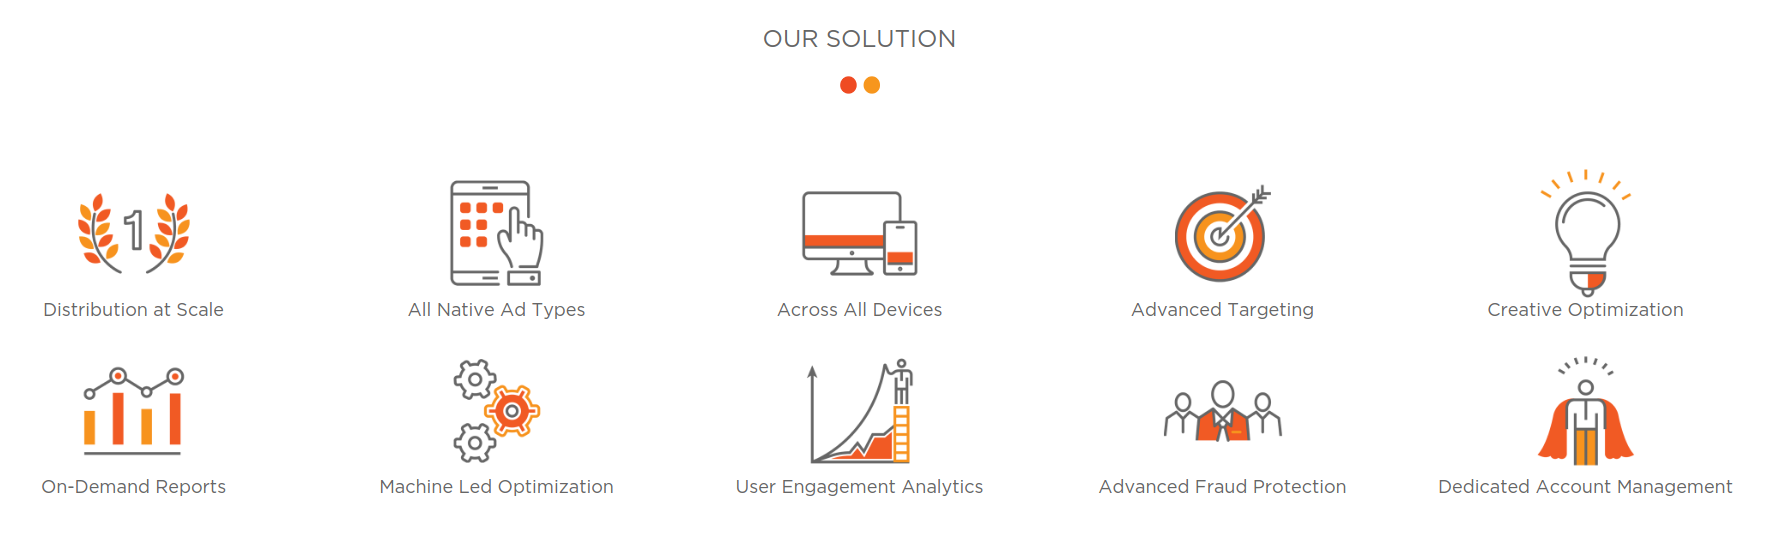
\includegraphics[width=\linewidth]{storygize.png}
\end{figure}

\begin{figure}
\caption{statistics on the har file produce, the 11/16/2017 at 14:11:37, with \textit{Chrome} \\ (http://www.softwareishard.com/blog/har-viewer/)}
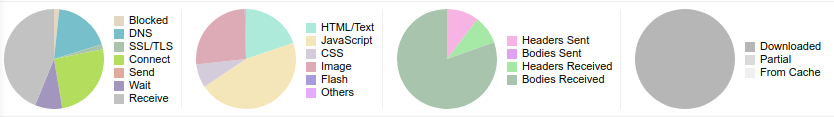
\includegraphics[width=\linewidth]{diags.png}
\end{figure}

\begin{figure}
\caption{statistics on the har file produce, the 11/28/2017 at 15:11:00, with \textit{Chrome} \\ (http://www.softwareishard.com/blog/har-viewer/)}
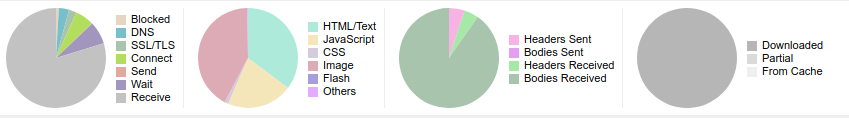
\includegraphics[width=\linewidth]{diags2.png}
\end{figure}


\begin{figure}
\caption{Content size by content type \\ 
Done with www.meta-chart.com \\ Data from tools.pingdom.com}
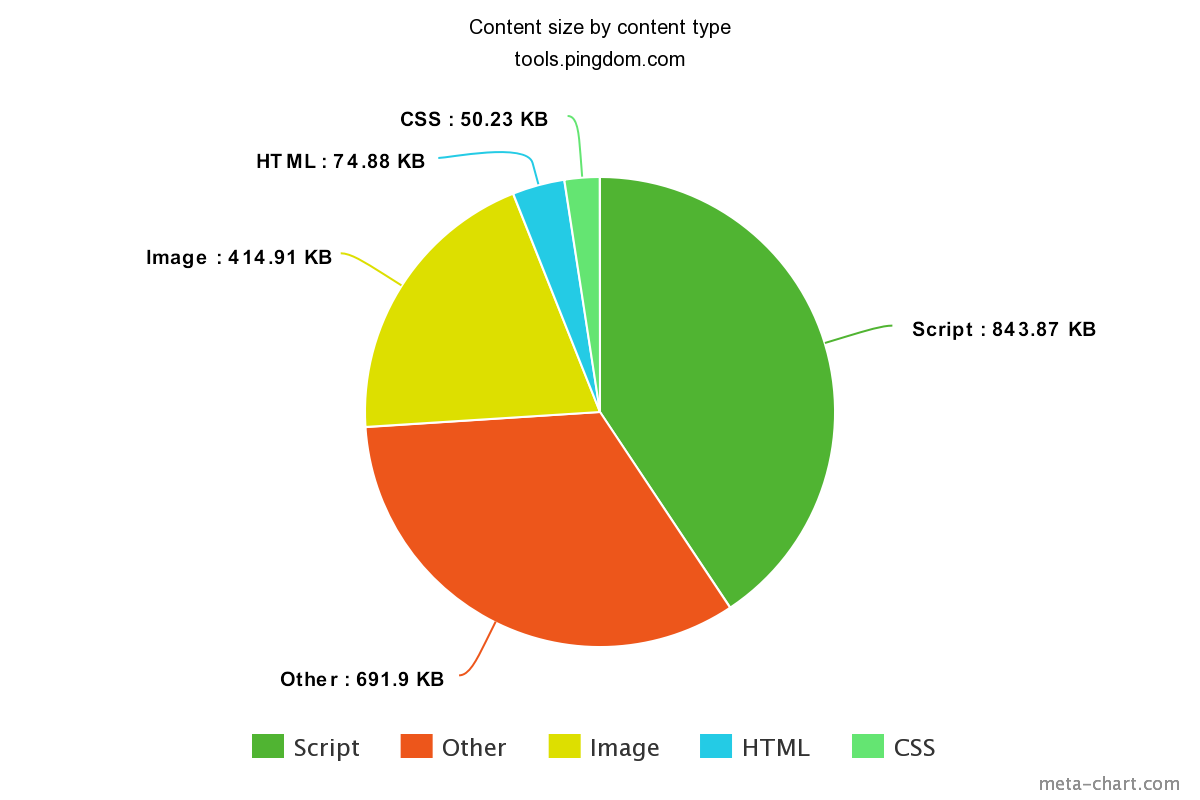
\includegraphics[width=\linewidth]{meta-chart.png}
\end{figure}


\begin{figure}
\caption{Requests by content type \\ 
Done with www.meta-chart.com \\ Data from tools.pingdom.com}
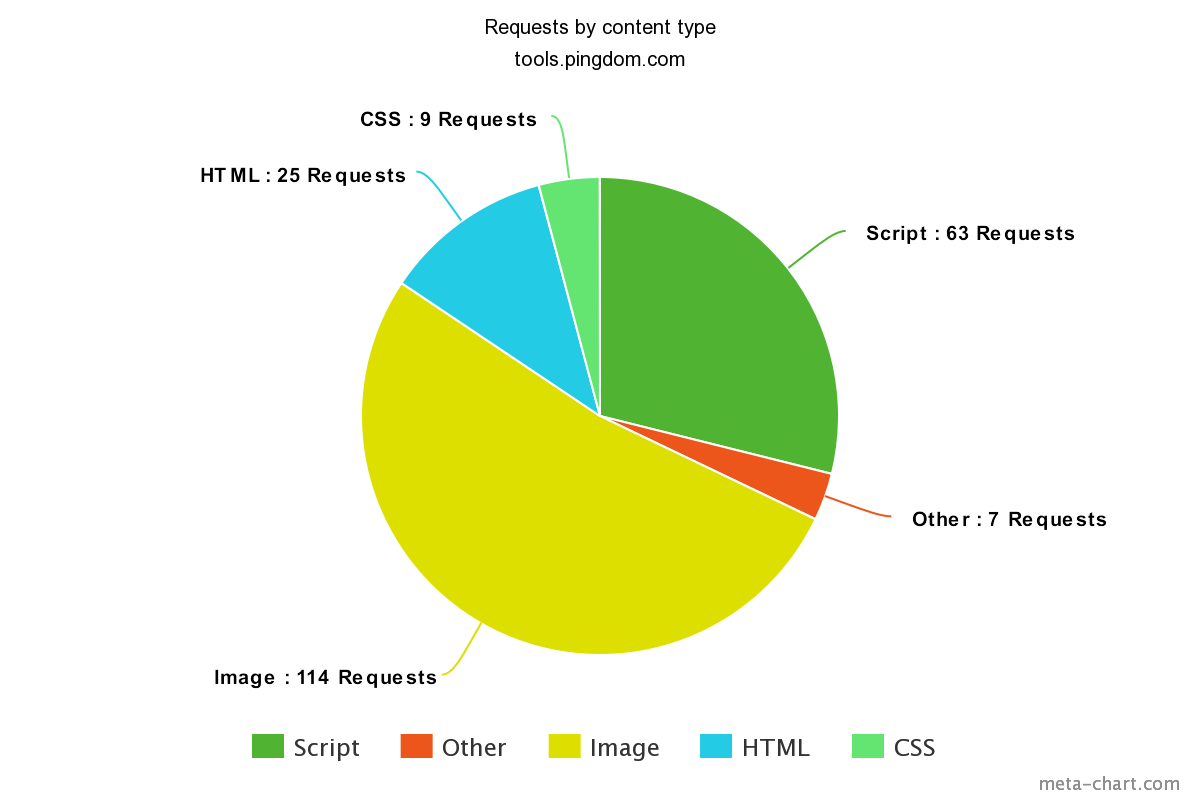
\includegraphics[width=\linewidth]{meta-chart1.png}
\end{figure}

\begin{figure}[ht!]
  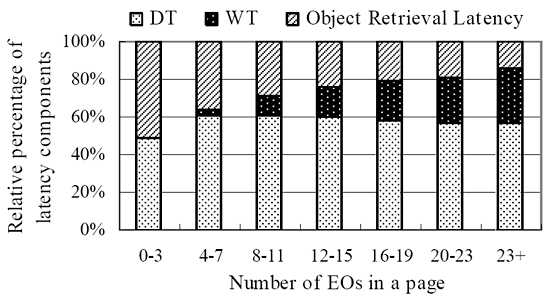
\includegraphics[width=\linewidth]{overhead.png}
  \caption{Figure II-3. Relative distribution of latency components showing that object overhead dominates web page latency. Website Optimization: Speed, Search Engine \& Conversion Rate Secrets by Andrew B. King}
\end{figure}

\begin{figure}[ht!]
  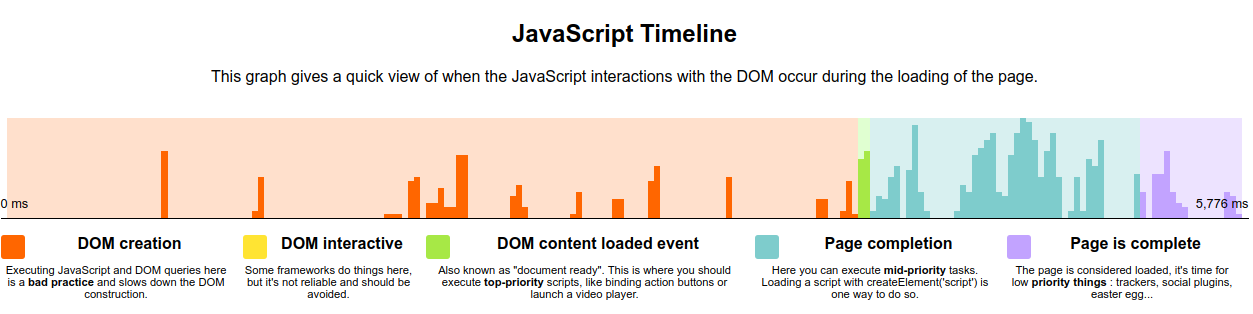
\includegraphics[width=\linewidth]{jsTimeline.png}
  \caption{http://yellowlab.tools analyze on bbc.com}
\end{figure}


\begin{figure}[ht!]
  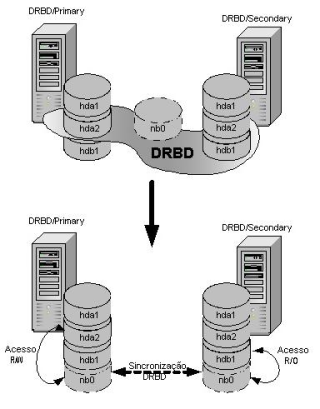
\includegraphics[width=\linewidth]{DRBD.png}
  \caption{DRBD concept overview \\ from https://upload.wikimedia.org/wikipedia/commons/5/5b/DRBD\_concept\_overview.png}
\end{figure}

\begin{figure}[ht!]
  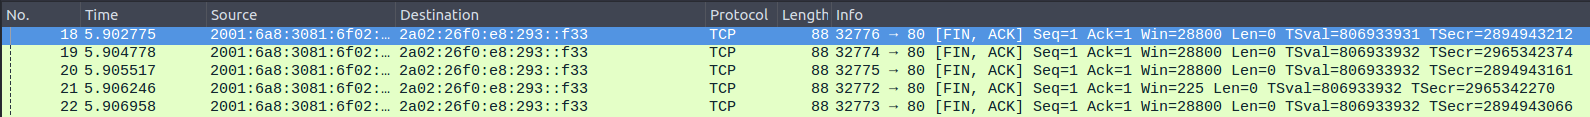
\includegraphics[width=\linewidth]{tcp.png}
  \caption{Akamai \textit{tcp} connection}
\end{figure}

\begin{figure}[ht!]
  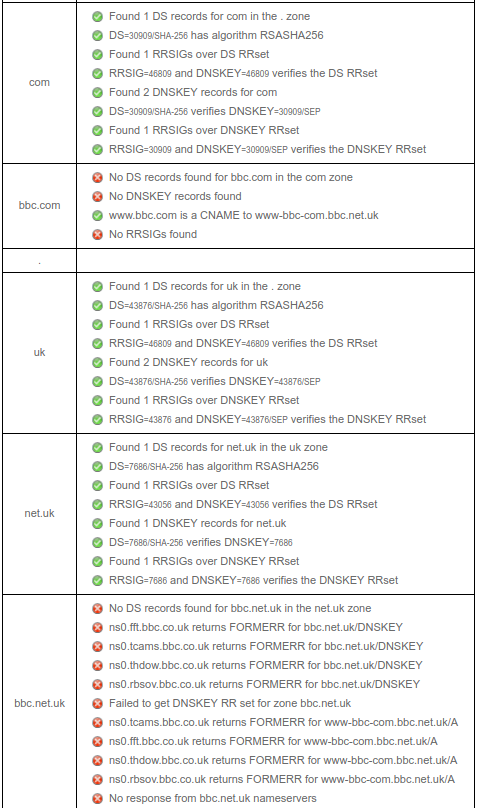
\includegraphics[width=\linewidth]{DNSSEC.png}
  \caption{http://dnssec-debugger.verisignlabs.com/www.bbc.com}
\end{figure}    


%https://

%TODO : 
%   - nbr of elements 
%   -list techno 

\end{document}